\documentclass{article}
\usepackage{amsmath,amssymb}
\usepackage[T1]{fontenc}
\usepackage[utf8]{inputenc}
\usepackage{textcomp}
\newcommand{\midtilde}{\raisebox{-0.25\baselineskip}{\textasciitilde}}
\usepackage{graphicx}
\usepackage{float}
\begin{document}

\section*{A Simple Example of Bayesian Networks} 

\textbf{1. The facts}\\
A is "Mike is not answering his phone" \\
B is "Mike is at home"\\
C is "It is raining"\\
\textbf{The fact dependencies} \\

\begin{figure}[H]
 \centering 
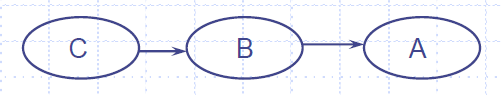
\includegraphics[scale=0.42]{images/mike-phone.png} 
 \caption{Directed graph - simple example}
 \label{fig:Mike}
\end{figure}
Note: C affects A indirectly in this case, so they can be treated as independent! \\
Let:
\begin{align*}
 P(A|B)& = 0.1 \\
 P(A|\midtilde B) & = 1 \\
P(B|C) & = 0.8 \\ 
P(B|\midtilde C) & = 0.5 \\
P(C) & = 0.6    \\
\end{align*}
from which we may further derive:
\begin{align*}
 P(\midtilde A|B)& = 0.9 \\
P(\midtilde B|C) & = 0.2 \\ 
P(\midtilde  B|\midtilde C) & = 0.5 \\
P(\midtilde  C) & = 0.4    \\
\end{align*}
\textbf{The probability that it is raining and Mike is at home but not answering the phone:} \\
\begin{align*}
p(A,B,C) & = p(A|B)p(B|C)p(C) \\
p(A,B,C) & = 0.1 * 0.8 * 0.6 \\
p(A,B,C) & = 0.048 \\
\end{align*}
Other possible calculations…\\
1. Calculate any of the dependent probabilities\\
\textbf{e.g. the probability that Mike is not answering the phone: P(A) = ?} \\
\begin{align*}
    p(A) & = p(A|B)p(B) + p(A|\midtilde B) p(\midtilde B) \\
\end{align*}
We have $p(A|B), p(A|\midtilde B)$, we don't have $p(B), p(\midtilde B)$.
\begin{align*}
    p(B) & = p(B|C)p(C) + p(B|\midtilde C)p(\midtilde C) \\
    p(B) & = 0.8*0.6 + 0.5*0.4 \\
    p(B) & = 0.68 \\
    p(\midtilde B) & = 0.32 \\
\end{align*}
Now we can solve:
\begin{align*}
    p(A) & = p(A|B)p(B) + p(A|\midtilde B) p(\midtilde B) \\
    p(A) & = 0.1*0.68+1*0.32 \\
    p(A) & = 0.388 \\
\end{align*}
2. Compute the probability of some event given the evidence\\
\textbf{e.g. the probability that it is raining given that Mike isn’t answering the phone: P(C|A) = ?} \\
\begin{align*}
    p(C|A) & = \frac{p(A,C)}{p(A)} \\
    % p(C|A) & = \frac{p(A|C)P(C)}{p(A)} \\
    % p(C|A) & = \frac{p(A|C)P(C)}{p(A)} \\
\end{align*}
%We have $p(C),p(A)$, we don't have $p(A|C)$. We derive it from the joint probability:
We have $p(A)$, we don't have $p(A,C)$:
\begin{align*}
    p(A,C) & = \sum_B p(A|B)p(B|C)p(C) \\
    p(A,C) & = p(A|B)p(B|C)p(C) + p(A|\midtilde B)p(\midtilde B|C)p(C) \\
    p(A,C) & = 0.1*0.8*0.6+1*0.2*0.6 \\
    p(A,C) & = 0.168 \\
    p(C|A) & = \frac{0.168}{0.388} \\
    p(C|A) & = 0.433 \\
\end{align*}
3. Compute the most likely set of events, given the evidence \\
\textbf{e.g. What is the most likely explanation for Mike not answering the phone?} Mike not answering the phone is the prior, so we want a likelihood (e.g. Mike is not at home) \textit{given Mike is not answering his phone...}, that is, given a prior.\\
\begin{align*}
p(B|A) & = \frac{p(A|B)p(B)}{p(A)} \\
p(B|A) & = \frac{0.1*0.68}{0.388} = 0.1753\\
p(\midtilde B|A) & = 1 - p(B|A) = \textbf{0.8247} \\
p(C|A) & = 0.433 \\
p(\midtilde C|A) & = 1 - p(C|A) = 0.567 \\
p(B,C|A) & = \frac{p(A,B,C)}{p(A)} = \frac{0.048}{0.388} = 0.1237 \\
p(\midtilde B, C|A) & = \frac{p(A,\midtilde B,C)}{p(A)}  = \frac{p(A|\midtilde B)p(\midtilde B|C) p(C)}{p(A)} = \frac{1*0.2*0.6}{0.388} = 0.3093\\
p(B, \midtilde C|A) & = \frac{p(A,B,\midtilde C)}{p(A)}  = \frac{p(A|B)p(B|\midtilde C) p(\midtilde C)}{p(A)} = \frac{0.1*0.5*0.4}{0.388} = 0.0515 \\
p(\midtilde B, \midtilde C | A) & = \frac{p(A,\midtilde B,\midtilde C)}{p(A)}  = \frac{p(A|\midtilde B)p(\midtilde B|\midtilde C) p(\midtilde C)}{p(A)} = \frac{1*0.5*0.4}{0.388} = 0.5155 \\
\end{align*}
The most likely explanation Mike is not answering the phone, is $p(\midtilde B|A)$, that is to say \textit{Mike is not at home, given he is not answering his phone}.

\end{document}
